\documentclass{standalone}
\usepackage{hsbcommon}
\begin{document}
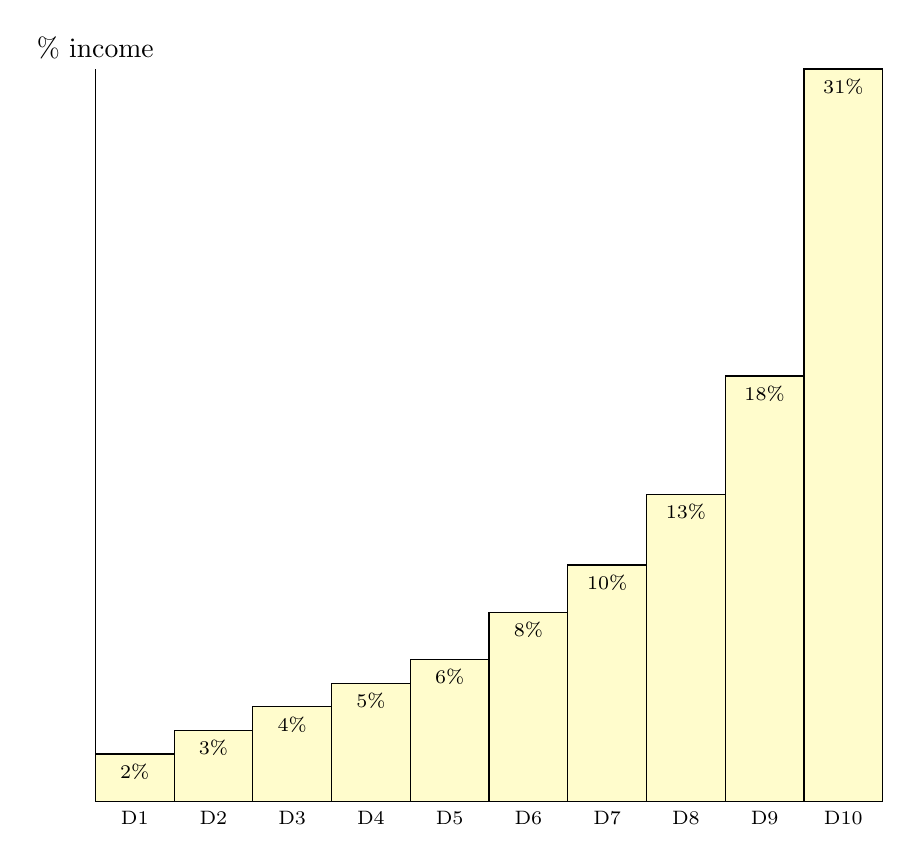
\begin{tikzpicture}[y=0.3cm]

    \tikzset{mystyle/.style={fill=yellow!20}}

    \draw (0,0) -- (10,0);
    \draw (0,0) -- (0,31) node[above] {\% income};

    \foreach [count=\i] \ii in {%
        2,
        3,
        4,
        5,
        6,
        8,
        10,
        13,
        18,
        31%
    }{
    \draw[mystyle] (\i-1,0) rectangle (\i,\ii);
    \node[below] at (\i-0.5,\ii) {\scriptsize \ii \%};
    \node[below] at (\i-0.5,0) {\scriptsize D\i};
    }

\end{tikzpicture}
\end{document}